\section{Tangent and Cotangent Spaces}
    \label{sec:tangent-cotangent}

    We now want to differentiate functions on a manifold. For temperature on
    Earth, this means choosing a direction of motion and measuring the rate
    of temperature change along it. Tangent spaces describe the possible
    directions, while cotangent spaces describe linear measurements of them.

    \subsection{Tangent Vectors as Velocities of Curves}
    Directional derivatives begin with a direction at a point. Let $p$ be a
    point on the sphere $S^2\subset\mathbb{R}^3$, and let $v\in\mathbb{R}^3$
    be a nonzero vector based at $p$ and lying in its geometric tangent plane.
    In ordinary multivariable calculus, we measure how a function changes
    along the straight line $p+tv$. But this line leaves the sphere as soon
    as $t\ne0$, so a function defined only on the sphere has no values there
    (Figure~\ref{fig:sphere_direction}).

    \begin{figure}[!ht]
        \centering
        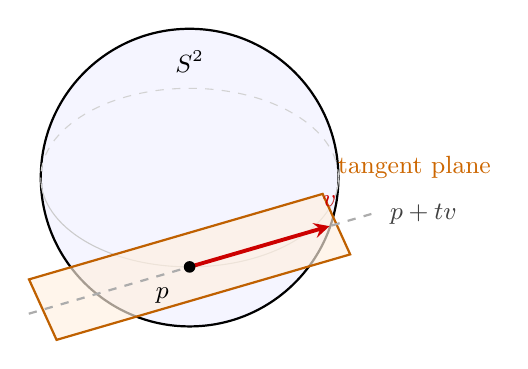
\begin{tikzpicture}[>=stealth, scale=1.05,
    x={(1.8cm,0cm)}, y={(0cm,1.44cm)}, z={(0cm,-1.08cm)}]
  % Use the same sphere projection as the curve-velocity figure.
  \draw[thick, fill=blue!4] (0,0) circle[radius=1.8cm];
  \draw[gray!35, dashed] (1.8cm,0cm) arc (0:180:1.8cm and 1.08cm);
  \draw[gray!40] (-1.8cm,0cm) arc (180:360:1.8cm and 1.08cm);
  \node[font=\small] at (0cm,1.4cm) {$S^2$};

  % The affine plane z=1 is tangent at p=(0,0,1).
  \filldraw[fill=orange!12, fill opacity=0.65,
      draw=orange!75!black, thick]
    (-0.894,-0.613,1) -- (1.079,0.105,1) --
    (0.894,0.613,1) -- (-1.079,-0.105,1) -- cycle;
  \node[font=\small, text=orange!80!black, above right=2pt]
    at (0.894,0.613,1) {tangent plane};

  % The tangent line lies in the plane and leaves the sphere away from p.
  \draw[gray!65, dashed, thick]
    ({-1.15*cos(20)},{-1.15*sin(20)},1) --
    ({1.30*cos(20)},{1.30*sin(20)},1)
    node[right=3pt, font=\small, text=black!75] {$p+tv$};
  \draw[->, red!80!black, line width=1.4pt]
    (0,0,1) -- ({cos(20)},{sin(20)},1)
    node[above=3pt, font=\small] {$v$};
  \fill (0,0,1) circle[radius=2pt];
  \node[font=\small, below left=4pt] at (0,0,1) {$p$};
\end{tikzpicture}

        \caption{%
            The vector $v$ lies in the tangent plane at $p$, but the straight
            line $p+tv$ leaves the sphere. To describe motion on the sphere,
            we use a curve on its surface.
        }
        \label{fig:sphere_direction}
    \end{figure}

    The idea is to replace the straight line $p+tv$ with a curve that stays
    on the manifold. On a smooth manifold $M$, consider a smooth curve
    \begin{equation}
        \gamma\colon(-\epsilon,\epsilon)\to M,\qquad\gamma(0)=p.
    \end{equation}
    Given a smooth function $f\colon M\to\mathbb{R}$, the composition is an
    ordinary function of one variable:
    \[
        f\circ\gamma\colon(-\epsilon,\epsilon)\to\mathbb{R},
        \qquad t\mapsto f(\gamma(t)).
    \]
    We can therefore measure how $f$ changes along the curve by taking
    \begin{equation}
        \left.\frac{d}{dt}\right|_{t=0}f(\gamma(t)).
    \end{equation}
    In the Euclidean case $M=\mathbb{R}^n$, choosing the straight-line curve
    $\gamma(t)=p+tv$ gives the familiar directional derivative:
    \begin{equation}
        \left.\frac{d}{dt}\right|_{t=0}f(\gamma(t))
        =\left.\frac{d}{dt}\right|_{t=0}f(p+tv)=D_vf(p).
    \end{equation}

    But there are many different smooth curves through $p$. An entire curve
    carries more
    information than we need: different paths can have the same initial
    direction and speed. We therefore group such curves together.
    Following Lee \cite[p.~72]{lee2013smooth}, we say two curves $\gamma_1$ and
    $\gamma_2$ are equivalent ($\gamma_1\sim\gamma_2$) if they produce the same
    rate of change for every smooth test function
    $f\colon M\to\mathbb{R}$:\footnote{%
        Lee discusses curve classes as an alternative to his definition using
        derivations, and uses smooth test functions defined near $p$.
        Multiplying such a function by a smooth bump function equal to $1$
        near $p$ and supported in its domain, then extending by zero, gives a
        global smooth function that agrees with it near $p$ and has the same
        derivatives along curves through $p$; see
        \cite[Proposition~2.25]{lee2013smooth}. Thus, the local and global
        test-function formulations are equivalent.}
    \begin{equation}
        \left.\frac{d}{dt}\right|_{t=0}f(\gamma_1(t))
        =\left.\frac{d}{dt}\right|_{t=0}f(\gamma_2(t)).
    \end{equation}
    Geometrically, the curves have the same initial velocity at $p$
    (Figure~\ref{fig:sphere_tangent}).

    \begin{figure}[!ht]
        \centering
        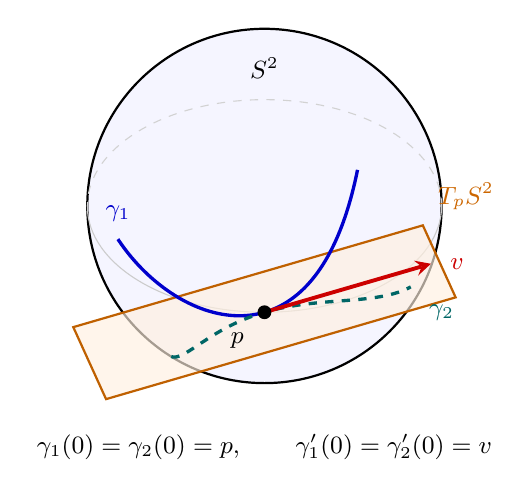
\begin{tikzpicture}[>=stealth, scale=1.25,
    x={(1.8cm,0cm)}, y={(0cm,1.44cm)}, z={(0cm,-1.08cm)}]
  % Orthographic projection of the unit sphere: (x,y,z) -> (1.8x,1.44y-1.08z).
  \draw[thick, fill=blue!4] (0,0) circle[radius=1.8cm];
  \draw[gray!35, dashed] (1.8cm,0cm) arc (0:180:1.8cm and 1.08cm);
  \draw[gray!40] (-1.8cm,0cm) arc (180:360:1.8cm and 1.08cm);
  \node[font=\small] at (0cm,1.4cm) {$S^2$};

  % A patch of the actual tangent plane z=1 at p=(0,0,1).
  \filldraw[fill=orange!12, fill opacity=0.65,
      draw=orange!75!black, thick]
    (-0.894,-0.613,1) -- (1.079,0.105,1) --
    (0.894,0.613,1) -- (-1.079,-0.105,1) -- cycle;
  \node[font=\small, text=orange!80!black, above right=2pt]
    at (0.894,0.613,1) {$T_pS^2$};

  % In a rotated tangent basis e1,e2, use
  % gamma_i(t)=t e1 +/- 0.85 t^2 e2 + sqrt(1-t^2-0.85^2 t^4) p.
  % Both lie on S^2, pass through p, and have derivative e1 at t=0.
  \draw[blue!80!black, very thick]
    plot[domain=-0.72:0.72, samples=101, variable=\t]
    ({cos(20)*\t-sin(20)*0.85*\t*\t},
     {sin(20)*\t+cos(20)*0.85*\t*\t},
     {sqrt(1-\t*\t-0.85*0.85*\t*\t*\t*\t)});
  \draw[teal!80!black, very thick, dashed]
    plot[domain=-0.72:0.72, samples=101, variable=\t]
    ({cos(20)*\t+sin(20)*0.85*\t*\t},
     {sin(20)*\t-cos(20)*0.85*\t*\t},
     {sqrt(1-\t*\t-0.85*0.85*\t*\t*\t*\t)});

  % Labels sit beside separated portions of the curves.
  \node[font=\small, text=blue!80!black, above=3pt]
    at (-0.827,0.168,0.537) {$\gamma_1$};
  \node[font=\small, text=teal!80!black, below right=3pt]
    at (0.827,-0.168,0.537) {$\gamma_2$};

  \draw[->, red!80!black, line width=1.4pt]
    (0,0,1) -- ({cos(20)},{sin(20)},1)
    node[right=3pt, font=\small] {$v$};
  \fill (0,0,1) circle[radius=2pt];
  \node[font=\small, below left=4pt] at (0,0,1) {$p$};
  \node[font=\small, align=center] at (0cm,-2.45cm)
    {$\gamma_1(0)=\gamma_2(0)=p,\qquad
       \gamma_1'(0)=\gamma_2'(0)=v$};
\end{tikzpicture}

        \caption{%
            Two distinct curves $\gamma_1$ and $\gamma_2$ pass through $p$
            with the same velocity vector, defining the same tangent vector
            $v=[\gamma_1]=[\gamma_2]\in T_pS^2$. The blue solid curve and
            green dashed curve take different paths but share the red
            velocity arrow at $p$.
        }
        \label{fig:sphere_tangent}
    \end{figure}

    \begin{definition}[Tangent Vector and Tangent Space \cite{lee2013smooth}]
        A \textbf{tangent vector} at $p\in M$ is an equivalence class of smooth
        curves through $p$, denoted $v=[\gamma]$. The \textbf{tangent space}
        $T_pM$ is the set of all such tangent vectors at $p$.
    \end{definition}

    Although adding curves directly on a curved manifold is not defined,
    $T_pM$ has the structure of an $n$-dimensional real vector space
    \cite[Problem~3-8, p.~76; Proposition~3.10, p.~57]{lee2013smooth}.
    When $M$ is a surface in $\mathbb{R}^3$, it is the familiar tangent plane
    drawn at $p$.

    For Euclidean space viewed as a manifold, we naturally identify
    \[
        T_p\mathbb{R}^n\cong\mathbb{R}^n.
    \]
    A vector $v\in\mathbb{R}^n$ is represented by the straight-line curve
    $\gamma(t)=p+tv$. This explains why an ordinary vector can serve as the
    direction of a directional derivative.

    \subsection{Cotangent Spaces}
    We have described directions of motion. Now we want to measure how a
    function changes in each direction. A rule that assigns a number to each
    tangent vector, linearly in that vector, is a \textbf{cotangent vector};
    that is, a linear map $T_pM\to\mathbb{R}$.
    The \textbf{cotangent space} $T_p^*M$ is the linear dual of the tangent
    space:\footnote{%
        Here, $\operatorname{Hom}_{\mathbb{R}}(T_pM,\mathbb{R})$ denotes the
        vector space of all linear maps from $T_pM$ to $\mathbb{R}$, the dual
        space recalled in Section~\ref{sec:preliminaries}.}
    \begin{equation}
        T_p^*M=\operatorname{Hom}_{\mathbb{R}}(T_pM,\mathbb{R}).
    \end{equation}
    A natural example is the \textbf{differential} of a smooth function
    $f\colon M\to\mathbb{R}$ at $p$. It measures the rate of change along a
    curve representing the tangent vector:
    \begin{equation}
        df_p([\gamma])=\left.\frac{d}{dt}\right|_{t=0}f(\gamma(t)).
    \end{equation}

    \paragraph{Intuition: $df_p$ Corresponds to the Gradient $\nabla f(p)$.}
    In multivariable calculus, the directional derivative can be calculated
    by taking the dot product of the gradient with a direction $v$. The vector
    $\nabla f(p)$ therefore determines a linear functional:
    \[
        \nabla f(p)\cdot(-)\colon\mathbb{R}^n\to\mathbb{R},
        \qquad v\mapsto\nabla f(p)\cdot v.
    \]
    Since $T_p\mathbb{R}^n$ is identified with $\mathbb{R}^n$, this functional
    is a cotangent vector. Choosing $\gamma(t)=p+tv$ in the manifold definition
    gives the same calculation:
    \begin{equation}
        df_p([\gamma])
        =\left.\frac{d}{dt}\right|_{t=0}f(p+tv)
        =\nabla f(p)\cdot v.
    \end{equation}
    Thus, $df_p$ is exactly the linear functional represented by the Euclidean
    gradient:
    \[
        df_p=\nabla f(p)\cdot(-).
    \]
